\documentclass[12pt]{ximera}
\title{Homework 3: Venn Diagrams and Inclusion-Exclusion}
\begin{document}
\begin{abstract}
Section 7.2: shading regions of a three-set Venn diagram, and using the Principle of
Inclusion-Exclusion to recover counts that were not given directly.
\end{abstract}
\maketitle

\section*{Section 7.2: Venn Diagrams and PIE}

\begin{problem}
For each of the following sets, sketch a Venn diagram with three sets $A$, $B$, and
$C$, and use shading to show the set. Sketch it on paper, then check yourself
against the solution.

\begin{prompt}
\textbf{(a)} $\olsi{A}\cap\left(B\cap C\right)$

\begin{freeResponse}
\end{freeResponse}

\begin{feedback}
Shade only the region that is inside \emph{both} $B$ and $C$ but outside $A$ ---
that is, the ``$B$ and $C$ overlap'' with the very center petal removed.
\begin{center}
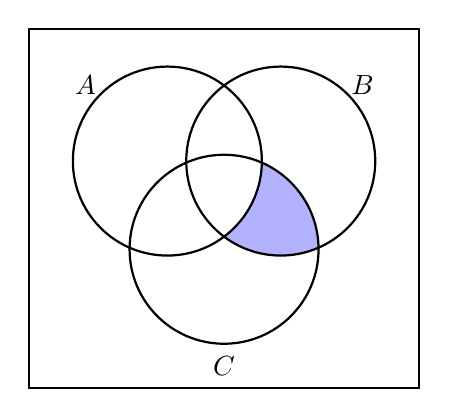
\begin{tikzpicture}[scale=0.8]
  \begin{scope}
    \clip (0.9,0.5) circle (1.5);
    \clip (0,-0.9) circle (1.5);
    \fill[blue!30,even odd rule] (-3.1,-3.1) rectangle (3.1,2.6) (-0.9,0.5) circle (1.5);
  \end{scope}
  \draw[thick] (-0.9,0.5) circle (1.5) node at (-2.2,1.7) {$A$};
  \draw[thick] (0.9,0.5) circle (1.5) node at (2.2,1.7) {$B$};
  \draw[thick] (0,-0.9) circle (1.5) node at (0,-2.75) {$C$};
  \draw[thick] (-3.1,-3.1) rectangle (3.1,2.6);
\end{tikzpicture}
\end{center}
\end{feedback}
\end{prompt}

\begin{prompt}
\textbf{(b)} $\left(A\cap\olsi{B}\right)\cup C$

\begin{freeResponse}
\end{freeResponse}

\begin{feedback}
Shade all of $C$, together with the part of $A$ that lies outside $B$. (The union
means you keep everything either piece covers.)
\begin{center}
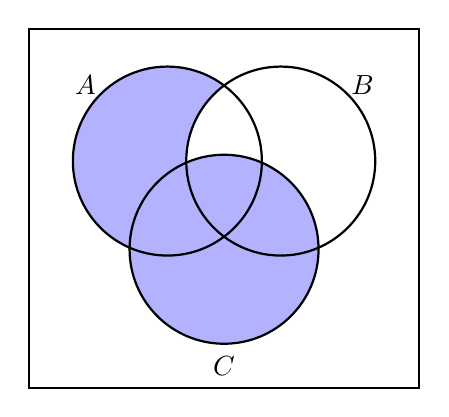
\begin{tikzpicture}[scale=0.8]
  \begin{scope}
    \clip (0,-0.9) circle (1.5);
    \fill[blue!30] (-3.1,-3.1) rectangle (3.1,2.6);
  \end{scope}
  \begin{scope}
    \clip (-0.9,0.5) circle (1.5);
    \fill[blue!30,even odd rule] (-3.1,-3.1) rectangle (3.1,2.6) (0.9,0.5) circle (1.5);
  \end{scope}
  \draw[thick] (-0.9,0.5) circle (1.5) node at (-2.2,1.7) {$A$};
  \draw[thick] (0.9,0.5) circle (1.5) node at (2.2,1.7) {$B$};
  \draw[thick] (0,-0.9) circle (1.5) node at (0,-2.75) {$C$};
  \draw[thick] (-3.1,-3.1) rectangle (3.1,2.6);
\end{tikzpicture}
\end{center}
\end{feedback}
\end{prompt}

\begin{prompt}
\textbf{(c)} $A\cap\left(B\cup\olsi{C}\right)$

\begin{freeResponse}
\end{freeResponse}

\begin{feedback}
Everything shaded must be inside $A$. Within $A$, keep the part that is in $B$
\emph{or} outside $C$. Equivalently, this set is
$\left(A\cap B\right)\cup\left(A\cap\olsi{C}\right)$: the only part of $A$ left
unshaded is the piece that is inside $C$ but outside $B$.
\begin{center}
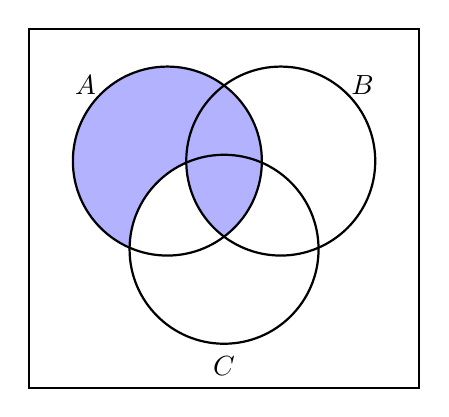
\begin{tikzpicture}[scale=0.8]
  \begin{scope}
    \clip (-0.9,0.5) circle (1.5);
    \clip (0.9,0.5) circle (1.5);
    \fill[blue!30] (-3.1,-3.1) rectangle (3.1,2.6);
  \end{scope}
  \begin{scope}
    \clip (-0.9,0.5) circle (1.5);
    \fill[blue!30,even odd rule] (-3.1,-3.1) rectangle (3.1,2.6) (0,-0.9) circle (1.5);
  \end{scope}
  \draw[thick] (-0.9,0.5) circle (1.5) node at (-2.2,1.7) {$A$};
  \draw[thick] (0.9,0.5) circle (1.5) node at (2.2,1.7) {$B$};
  \draw[thick] (0,-0.9) circle (1.5) node at (0,-2.75) {$C$};
  \draw[thick] (-3.1,-3.1) rectangle (3.1,2.6);
\end{tikzpicture}
\end{center}
\end{feedback}
\end{prompt}
\end{problem}

\begin{problem}
Use the Principle of Inclusion-Exclusion to solve the following.

If $|A|=12$, $|B|=27$, and $|A\cup B|=30$, what is $|A\cap B|$?

$|A\cap B| = \answer{9}$

\begin{hint}
The Principle of Inclusion-Exclusion for two sets says
$|A\cup B|=|A|+|B|-|A\cap B|$. Everything but $|A\cap B|$ is known.
\end{hint}

\begin{feedback}
By inclusion-exclusion,
\[ |A\cup B| = |A|+|B|-|A\cap B|, \]
so
\[ 30 = 12+27-|A\cap B| = 39 - |A\cap B|, \]
which gives $|A\cap B|=39-30=9$.

The reason for the subtraction: adding $|A|$ and $|B|$ counts everything in the
overlap twice, so you remove one of those copies.
\end{feedback}
\end{problem}

\begin{problem}
Sketch a Venn diagram and use it to solve the following.

Suppose $140$ people are interviewed about their cooking habits, with the following
results:
\begin{itemize}
    \item $63$ use electric ranges;
    \item $58$ use gas ranges;
    \item $19$ use microwave ovens and electric ranges;
    \item $17$ use microwave ovens and gas ranges;
    \item $4$ use both electric and gas ranges;
    \item $1$ uses all three;
    \item $2$ use none of the three.
\end{itemize}

\begin{prompt}
How many people surveyed use only microwave ovens in their cooking?

$\answer{21}$ people.

\begin{hint}
First find $|M|$, the total number of microwave users, using inclusion-exclusion on
all three sets --- you know that $140-2=138$ people use at least one of the three.
Then peel off the parts of $M$ that overlap $E$ or $G$.
\end{hint}

\begin{feedback}
Since $2$ people use none of the three, the number using at least one is
$|M\cup E\cup G|=140-2=138$.

Inclusion-exclusion for three sets gives
\[
|M\cup E\cup G|=|M|+|E|+|G|-|M\cap E|-|M\cap G|-|E\cap G|+|M\cap E\cap G|,
\]
so
\[
138 = |M| + 63 + 58 - 19 - 17 - 4 + 1 = |M| + 82,
\]
giving $|M|=56$.

Now split $M$ into its four regions. Of the $19$ who use a microwave and an electric
range, $1$ uses all three, so $18$ use exactly the microwave and electric range.
Likewise $17-1=16$ use exactly the microwave and gas range, and $1$ uses all three.
So the ``microwave only'' region contains
\[ 56 - 18 - 16 - 1 = 21 \]
people.
\end{feedback}
\end{prompt}
\end{problem}

\end{document}
